%\documentclass[a4paper,10pt]{article}
%\usepackage{a4}
\documentclass[10pt]{article}
\usepackage{amsfonts}
\usepackage{amsthm}
\usepackage{amssymb}
\usepackage{graphicx, enumerate}
\usepackage{amsmath}
\usepackage{latexsym}
\usepackage{longtable}
\usepackage{tabularx}
\usepackage{setspace}
\usepackage{float}
\usepackage{rotating}
\usepackage{tikz}
\usepackage{verbatim}
\usepackage{xcolor}
\usetikzlibrary{calc}
\usepackage{caption}


%\begin{comment}
\newtheorem{theorem}{Theorem}[section]
%\newtheorem{thm}[theorem]{Theorem}%[section]
%\newtheorem{cl}[theorem]{Claim}
\newtheorem{lemma}[theorem]{Lemma}
\newtheorem{prop}[theorem]{Proposition}
%\newtheorem{oprb}[theorem]{Open Problem}
\newtheorem*{oprb}{Open Problem}
\newtheorem{obs}[theorem]{Observation}
%\newtheorem{cor}[theorem]{Corollary}
%\newtheorem{conj}[theorem]{Conjecture}
\newtheorem{const}[theorem]{Construction}
%\newtheorem{dfn}[theorem]{Definition}
%\newtheorem{dfn}[theorem]{Definition}
\newtheorem{exm}[theorem]{Example}
%\newtheorem{prm}[theorem]{Problem}
\newtheorem{rem}[theorem]{Remark}
\newtheorem*{rem*}{Remark}


\theoremstyle{definition}
\newtheorem{definition}[theorem]{Definition}

%\end{comment}



\newcommand{\rd}{{\rm d}}
\newcommand{\dist}{{\rm{dist}}}


\def\amb{\allowbreak}
\def\ni{\noindent}
\footskip=30pt
\vspace{5cm}
%\begin{document}


%colors
\definecolor{darkpastelgreen}{rgb}{0.01, 0.75, 0.24}
\definecolor{blue-violet}{rgb}{0.54, 0.17, 0.89}
\definecolor{dgreen}{RGB}{20,100,10}

\newcommand{\bblue}[1]{{\color{blue}{#1}}}
\newcommand{\ggreen}[1]{{\color{green}{#1}}}
\newcommand{\dpgreen}[1]{{\color{darkpastelgreen}{#1}}}
\newcommand{\rred}[1]{{\color{red}{#1}}}
\newcommand{\mmag}[1]{{\color{magenta}{#1}}}
\newcommand{\bv}[1]{{\color{blue-violet}{#1}}}


\newcommand{\dal}[1]{\par\vskip2mm\noindent\bblue{Dalibor: #1}\par\noindent}
\newcommand{\syl}[1]{\par\vskip2mm\noindentGreen{Sylwia: #1}\par\noindent}
\marginparwidth1.5in
%need to do \margbl{}{my own text} at least in some installations --- leave blank {} right after command



\newcommand{\dalb}[1]{\par\vskip2mm\noindent\bblue{Dalibor: #1}\par\noindent}
\newcommand{\dalr}[1]{\par\vskip2mm\noindent\rred{Dalibor: #1}\par\noindent}
\newcommand{\dalm}[1]{\par\vskip2mm\noindent\mmag{Dalibor: #1}\par\noindent}
\newcommand{\dalgr}[1]{\par\vskip2mm\noindent\dpgreen{Dalibor: #1}\par\noindent}
\newcommand{\dalbv}[1]{\par\vskip2mm\noindent\bv{Dalibor: #1}\par\noindent}


%http://joshua.smcvt.edu/latex2e/_005cnewcommand-_0026-_005crenewcommand.html

\marginparwidth1.3in
\newcommand{\margbl}[1]{\marginpar{\textcolor{blue}{#1}}}
\newcommand{\margred}[1]{\marginpar{\textcolor{red}{#1}}}
\newcommand{\marggr}[1]{\marginpar{\textcolor{green}{#1}}}

%\usepackage{parskip}

\newcommand{\GG}{\ensuremath{\mathcal{G}}}
\parindent0pt
\parskip4pt
\begin{document}


\textwidth4.5true in
\textheight7.2true in


\section{Catalog}\label{sec:catalog}

\vspace{30pt}
    % Left graph of the first pair
    \begin{minipage}{0.48\textwidth}
        \centering
        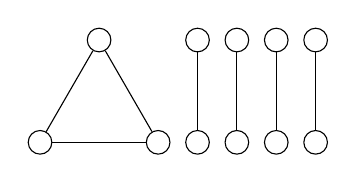
\begin{tikzpicture}[scale=0.5]
            \tikzstyle{every node}=[draw,circle, minimum size=3mm, inner sep=0pt]
            \draw [circle] (0,0) node (0) {};
            \node (11) at (-120:3cm) {};
            \node (6) at (-60:3cm) {};
            \draw (0)--(11);
            \draw (0)--(6);
            \draw (11)--(6);
            % Sticks
            \node (7) at ($(0) + (2.5, 0)$) {};
            \node (4) at ($(6) + (1, 0)$) {};
            \draw (7)--(4);
            \node (1) at ($(0) + (3.5, 0)$) {};
            \node (10) at ($(6) + (2, 0)$) {};
            \draw (10)--(1);
            \node (3) at ($(0) + (4.5, 0)$) {};
            \node (2) at ($(6) + (3, 0)$) {};
            \draw (2)--(3);
            \node (12) at ($(0) + (5.5, 0)$) {};
            \node (5) at ($(6) + (4, 0)$) {};
            \draw (5)--(12);
        \end{tikzpicture}
        \captionof{figure}{$G_{1}$}
        \label{fig:G1}
    \end{minipage}\hfill%
    % Right graph of the first pair
    \begin{minipage}{0.49\textwidth}
        \centering
        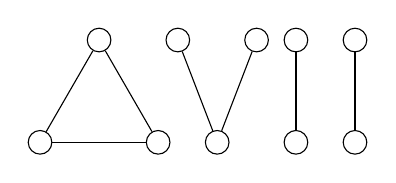
\begin{tikzpicture}[scale=0.5]
            \tikzstyle{every node}=[draw,circle,minimum size=3mm, inner sep=0pt]
            \draw (0,0) node (02) {};
            \node (112) at (-120:3cm) {};
            \node (62) at (-60:3cm) {};
            \draw (02)--(112);
            \draw (02)--(62);
            \draw (112)--(62);
            \node (42) at ($(62) + (1.5, 0)$) {};
            \node (72) at ($(02) + (2,0)$) {};
            \node (52) at ($(72) + (2,0)$) {};
            \draw (42)--(72);
            \draw (42)--(52);
            \node (1b) at ($(42) + (2, 0)$) {};
            \node (10b) at ($(52) + (1, 0)$) {};
            \draw (10b)--(1b);
            \node (92) at ($(10b) + (1.5, 0)$) {};
            \node (22) at ($(1b) + (1.5, 0)$) {};
            \draw (22)--(92);
        \end{tikzpicture}
        \captionof{figure}{$G_{2}$}
        \label{fig:G2}
    \end{minipage}

\vspace{1cm}
% G3,G4%%%%%%%%%%%%%%%%%%%%%%%%%%%%%%%%%%%%%%%%%%%%%%%%%%%%%%%%%%%%%%%%%%%%%%%%%%%

\begin{minipage}{0.48\textwidth}
    \centering
    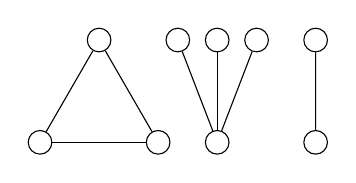
\begin{tikzpicture}[scale=0.5]
        \tikzstyle{every node}=[draw,circle,minimum size=3mm, inner sep=0pt]
        \draw (0,0) node (0) {};
        \node (11) at (-120:3cm) {};
        \node (6) at (-60:3cm) {};
        \draw (0)--(11);
        \draw (0)--(6);
        \draw (11)--(6);
        % Sticks and other nodes
        \node (1) at ($(6) + (1.5, 0)$) {};
        \node (2) at ($(0) + (3, 0)$) {};
        \node (4) at ($(2) + (-1,0)$) {};
        \node (8) at ($(2) + (1,0)$) {};
        \draw (1)--(4);
        \draw (1)--(2);
        \draw (1)--(8);
        \node (12) at ($(8) + (1.5, 0)$) {};
        \node (3) at ($(6) + (4, 0)$) {};
        \draw (3)--(12);
    \end{tikzpicture}
    \captionof{figure}{$G_3$}
    \label{fig:G3}
\end{minipage}\hfill % Space between minipages
\begin{minipage}{0.48\textwidth}
    \centering
    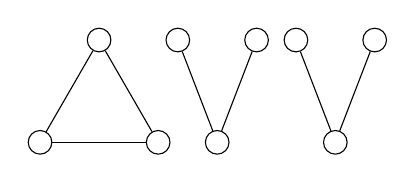
\begin{tikzpicture}[scale=0.5]
        \tikzstyle{every node}=[draw,circle,minimum size=3mm, inner sep=0pt]
        \draw (0,0) node (02) {};
        \node (112) at (-120:3cm) {};
        \node (62) at (-60:3cm) {};
        \draw (02)--(112);
        \draw (02)--(62);
        \draw (112)--(62);
        % Additional structures
        \node (32) at ($(62) + (1.5, 0)$) {};
        \node (122) at ($(02) + (2,0)$) {};
        \node (22) at ($(122) + (2,0)$) {};
        \draw (32)--(122);
        \draw (32)--(22);
        \node (1b) at ($(32) + (3, 0)$) {};
        \node (42) at ($(22) + (1,0)$) {};
        \node (82) at ($(42) + (2,0)$) {};
        \draw (1b)--(42);
        \draw (1b)--(82);
    \end{tikzpicture}
    \captionof{figure}{$G_4$}
    \label{fig:G4}
\end{minipage}

\vspace{1cm}

%G5%%%%%%%%%%%%%%%%%%%%%%%%%%%%%%%%%%%%%%%%%%%%%%%%%%%%%%%%%%%%%%%%%%%%%%%%%%%%%%%
\begin{minipage}{0.48\textwidth}
    \centering
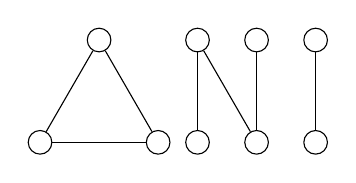
\begin{tikzpicture}[scale=0.5]
    \tikzstyle{every node}=[draw,circle,minimum size=3mm,inner sep=0pt]

    \draw (0,0) node (02) {};
    \node (112) at (-120:3cm) {};
    \node  (62) at (-60:3cm) {};

    \draw (02)--(112) {};
    \draw (02)--(62) {};
    \draw (112)--(62) {};

    % Repeat of additional line segments
    \node (32) at ($(02) + (2.5, 0)$) {};
    \node (122) at ($(62) + (1,0)$) {};
    \node  (22) at ($(32) + (-60:3cm)$) {};
    \node  (92) at ($(32) + (1.5,0)$) {};
    \draw (32)--(122) {};
    \draw (32)--(22) {};
    \draw (92)--(22) {};

    \node (42) at ($(92) + (1.5, 0)$) {};
    \node (1b) at ($(22) + (1.5, 0)$) {};
    \draw (42)--(1b) {};

\end{tikzpicture}
\captionof{figure}{$G_{5}$}
\label{fig:G5}
\end{minipage}
\hfill
\begin{minipage}{0.48\textwidth}
    \centering
    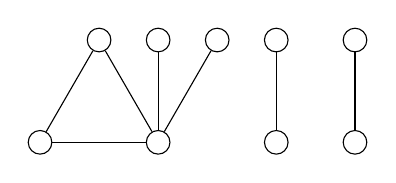
\begin{tikzpicture}[scale=0.5]
        \tikzstyle{every node}=[draw,circle,minimum size=3mm, inner sep=0pt]
        \node (11) at (0,0) {};
        \node (12) at (-120:3cm) {};
        \node (13) at (-60:3cm) {};
        \node (14) at ($(11)+(1.5,0)$) {};
        \node (15) at ($(14)+(1.5,0)$) {};
        
        \draw (11) to (12);
        \draw (11) to (13);
        \draw (12) to (13);
               
        \node (16) at ($(15)+(1.5, 0)$) {};
        \node (17) at ($(13)+(3, 0)$) {};
        \node (18) at ($(16)+(2, 0)$) {};
        \node (19) at ($(17)+(2, 0)$) {};
        
        \draw (13) to (14);
        \draw (13) to (15);
        \draw (16) to (17);
        \draw (18) to (19);
    \end{tikzpicture}
    \captionof{figure}{$G_6$}
\end{minipage}
\vspace{1cm}

\begin{minipage}{0.48\textwidth}
    \centering
    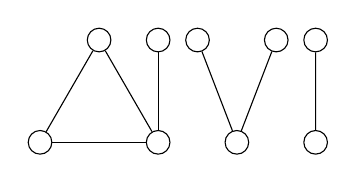
\begin{tikzpicture}[scale=0.5]
    \tikzstyle{every node}=[draw,circle,minimum size=3mm, inner sep=0pt]
    \node (11) at (0,0) {};
    \node (12) at (-120:3cm) {};
    \node (13) at (-60:3cm) {};
    \node (14) at ($(11)+(1.5,0)$) {};
    
    \draw (11) to (12);
    \draw (12) to (13);
    \draw (13) to (11);
    \draw (14) to (13);
    
    \node (15) at ($(13) + (2,0)$) {};
    \node (16) at ($(14) + (1,0)$) {};
    \node (17) at ($(16) + (2,0)$) {};
    \node (18) at ($(15)+ (2,0)$) {};
    \node (19) at ($(17)+ (1,0)$) {};
    
    \draw (15) to (16);
    \draw (15) to (17);
    \draw (19) to (18);
\end{tikzpicture}
\captionof{figure}{$G_7$}
\end{minipage}
\hfill
\begin{minipage}{0.48\textwidth}
    \centering
    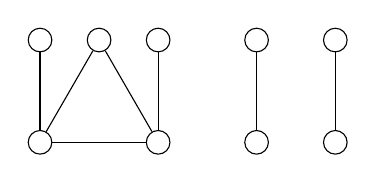
\begin{tikzpicture}[scale=0.5]
        \tikzstyle{every node}=[draw,circle,minimum size=3mm, inner sep=0pt]
        \node (11) at (0,0) {};
        \node (12) at (-120:3cm) {};
        \node (13) at (-60:3cm) {};
        \node (14) at ($(11)+(-1.5,0)$) {};
        \node (15) at ($(11)+(1.5,0)$) {};
        
        \draw (11) to (12);
        \draw (11) to (13);
        \draw (12) to (13);
               
        \node (16) at ($(15)+(2.5, 0)$) {};
        \node (17) at ($(13)+(2.5, 0)$) {};
        \node (18) at ($(16)+(2, 0)$) {};
        \node (19) at ($(17)+(2, 0)$) {};
        
        \draw (12) to (14);
        \draw (13) to (15);
        \draw (16) to (17);
        \draw (18) to (19);
    \end{tikzpicture}
    \captionof{figure}{$G_8$}
\end{minipage}
\vspace{1cm}

\begin{minipage}{0.48\textwidth}
    \centering
    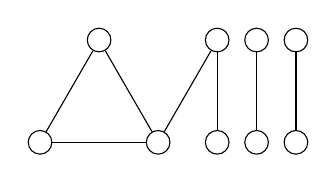
\begin{tikzpicture}[scale=0.5]
        \tikzstyle{every node}=[draw,circle,minimum size=3mm, inner sep=0pt]
        \node (11) at (0,0) {};
        \node (12) at (-120:3cm) {};
        \node (13) at (-60:3cm) {};
        \node (14) at ($(11)+(3,0)$) {};
        \node (15) at ($(13)+(1.5,0)$) {};
        
        \draw (11) to (12);
        \draw (11) to (13);
        \draw (12) to (13);
               
        \node (16) at ($(14)+(1, 0)$) {};
        \node (17) at ($(15)+(1, 0)$) {};
        \node (18) at ($(16)+(1, 0)$) {};
        \node (19) at ($(17)+(1, 0)$) {};
        
        \draw (13) to (14);
        \draw (14) to (15);
        \draw (16) to (17);
        \draw (18) to (19);
    \end{tikzpicture}
    \captionof{figure}{$G_9$}
\end{minipage}
\hfill
\begin{minipage}{0.48\textwidth}
    \centering
    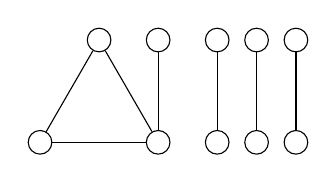
\begin{tikzpicture}[scale=0.5]
        \tikzstyle{every node}=[draw,circle,minimum size=3mm, inner sep=0pt]
        \node (11) at (0,0) {};
        \node (12) at (-120:3cm) {};
        \node (13) at (-60:3cm) {};
        \node (14) at ($(11)+(1.5,0)$) {};
        
        \draw (11) to (12);
        \draw (11) to (13);
        \draw (12) to (13);
            
        \node (15) at ($(14)+(1.5,0)$) {};
        \node (16) at ($(13)+(1.5,0)$) {};

        \node (17) at ($(15)+(1,0)$) {};
        \node (18) at ($(16)+(1,0)$) {};

        \node (19) at ($(17)+(1,0)$) {};
        \node (20) at ($(18)+(1,0)$) {};
        
        \draw (13) to (14);
        \draw (15) to (16);
        \draw (17) to (18);
        \draw (19) to (20);
    \end{tikzpicture}
    \captionof{figure}{$G_{10}$}
\end{minipage}
\vspace{1cm}

\begin{minipage}{0.48\textwidth}
    \centering
    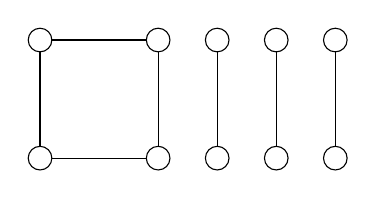
\begin{tikzpicture}[scale=0.5]
        \tikzstyle{every node}=[draw,circle,minimum size=3mm, inner sep=0pt]
            \node (S1) at (0,0) {};
            \node (S2) at ($(S1)+(3, 0)$) {};
            \node (S3) at ($(S2)+(0, -3)$) {};
            \node (S4) at ($(S1)+(0, -3)$) {};

            \node (1P1) at ($(S2)+(1.5, 0)$) {};
            \node (1P2) at ($(S3)+(1.5, 0)$) {};

            \node (2P1) at ($(1P1)+(1.5, 0)$) {};
            \node (2P2) at ($(1P2)+(1.5, 0)$) {};

            \node (3P1) at ($(2P1)+(1.5, 0)$) {};
            \node (3P2) at ($(2P2)+(1.5, 0)$) {};
            
            \draw (S1) -- (S2) -- (S3) -- (S4) -- (S1);

            \draw (1P1) -- (1P2);
            \draw (2P1) -- (2P2);
            \draw (3P1) -- (3P2);

        \end{tikzpicture}
    \captionof{figure}{$G_{11}$}
\end{minipage}
\hfill
\begin{minipage}{0.48\textwidth}
    \centering
    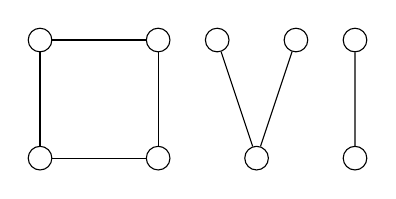
\begin{tikzpicture}[scale=0.5]
        \tikzstyle{every node}=[draw,circle,minimum size=3mm, inner sep=0pt]
            \node (S1) at (0,0) {};
            \node (S2) at ($(S1)+(3, 0)$) {};
            \node (S3) at ($(S2)+(0, -3)$) {};
            \node (S4) at ($(S1)+(0, -3)$) {};

            \node (1P1) at ($(S2)+(1.5, 0)$) {};
            \node (1P2) at ($(S3)+(2.5, 0)$) {};
            \node (1P3) at ($(1P1)+(2, 0)$) {};


            \node (2P1) at ($(1P3)+(1.5, 0)$) {};
            \node (2P2) at ($(1P2)+(2.5, 0)$) {};
            
            \draw (S1) -- (S2) -- (S3) -- (S4) -- (S1);

            \draw (1P1) -- (1P2) -- (1P3);
            \draw (2P1) -- (2P2);

        \end{tikzpicture}
    \captionof{figure}{$G_{12}$}
\end{minipage}
\vspace{1cm}

\begin{minipage}{0.48\textwidth}
    \centering
    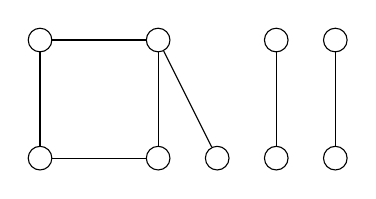
\begin{tikzpicture}[scale=0.5]
        \tikzstyle{every node}=[draw,circle,minimum size=3mm, inner sep=0pt]
            \node (S1) at (0,0) {};
            \node (S2) at ($(S1)+(3, 0)$) {};
            \node (S3) at ($(S2)+(0, -3)$) {};
            \node (S4) at ($(S1)+(0, -3)$) {};
            \node (SL1) at ($(S3)+(1.5, 0)$) {};

            \node (1P2) at ($(S2)+(3, 0)$) {};
            \node (1P1) at ($(SL1)+(1.5, 0)$) {};

            \node (2P1) at ($(1P1)+(1.5, 0)$) {};
            \node (2P2) at ($(1P2)+(1.5, 0)$) {};
            
            \draw (S1) -- (S2) -- (S3) -- (S4) -- (S1);
            \draw (S2) -- (SL1);

            \draw (1P1) -- (1P2);
            \draw (2P1) -- (2P2);

        \end{tikzpicture}
    \captionof{figure}{$G_{10}$}
\end{minipage}
\hfill
\begin{minipage}{0.48\textwidth}
    \centering
    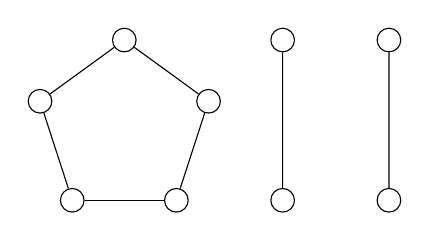
\begin{tikzpicture}[scale=0.9]
        \tikzstyle{every node}=[draw,circle,minimum size=3mm, inner sep=0pt]
    
    \def\radius{1.25}
    
    \node (A) at ({\radius*cos(90)}, {\radius*sin(90)}) {}; % Top vertex
    \node (B) at ({\radius*cos(162)}, {\radius*sin(162)}) {};
    \node (C) at ({\radius*cos(234)}, {\radius*sin(234)}) {};
    \node (D) at ({\radius*cos(306)}, {\radius*sin(306)}) {};
    \node (E) at ({\radius*cos(18)},{\radius*sin(18)}) {}; 

    \draw (A) -- (B);
    \draw (B) -- (C);
    \draw (C) -- (D);
    \draw (D) -- (E);
    \draw (E) -- (A);

    % Add extra nodes and edges
    \node (F) at ($(D) + (1.5, 0)$) {}; % Additional node near C
    \node (G) at ($(F) + (0, 2.261)$) {};
    \node (H) at ($(D) + (3, 0)$) {}; % Additional node near E
    \node (I) at ($(H) + (0, 2.261)$) {};

    % Additional edges
    \draw (F) -- (G);
    \draw (H) -- (I);

    % Add label below
\end{tikzpicture}

    \captionof{figure}{$G_{10}$}
\end{minipage}

\newpage
\section{Labelings}\label{sec:another}
For each $G_{i}$ we provide a $\rho$-tripartite labeling on the left and a $1$-rotational $\rho$-tripartite labeling on the right.
\begin{figure}[ht]
    \centering
\begin{tikzpicture}[scale=0.6]

    % C_{3}
    \node[draw,circle] (0) at (0,0) {0};
    \node[draw, circle]  (6) at (-60: 3 cm) {6};
    \node[draw, circle] (11) at ($(6) + (-120:3cm)$) {13};

    \draw (0)--(11) node [draw = none, midway,left,sloped, fill = none, rotate=90] {$2$};
    \draw (0)--(6) node [draw = none, midway,above right,sloped, fill = none, rotate=60] {$6$};
    \draw (11)--(6) node [draw = none, midway,below right,sloped, fill = none, rotate=-60] {$7(7)$};
    % sticks
% Adding three line segments with nodes
\node[draw, circle] (7) at ($(6) + (1.5, 0)$) {12};
\node[draw, circle] (4) at ($(0) + (3, 0)$) {7};
\draw (7)--(4) node [draw = none, midway,left,sloped, fill = none, rotate=90] {$5$};

\node[draw, circle] (1) at ($(4) + (1.5, 0)$) {5};
\node[draw, circle] (10) at ($(7) + (1.5, 0)$) {9};
\draw (10)--(1) node [draw = none, midway, left,sloped, fill = none, rotate=90] {$4$};

\node[draw, circle] (3) at ($(10) + (1.5, 0)$) {11};
\node[draw, circle] (2) at ($(1) + (1.5, 0)$) {8};
\draw (2)--(3) node [draw = none, midway,left,sloped, fill = none, rotate=90] {$3$};

\node[draw, circle] (12) at ($(3) + (1.5, 0)$) {2};
\node[draw, circle] (5) at ($(2) + (1.5, 0)$) {1};
\draw (5)--(12) node [draw = none, midway,left,sloped, fill = none, rotate=90] {$1$};

\begin{scope}[shift={(13,0)}] % shift right
    \node[draw,circle] (0) at (0,0) {0};
    \node[draw, circle]  (6) at (-60: 3 cm) {6};
    \node[draw, circle] (11) at ($(6) + (-120:3cm)$) {11};

    \draw (0)--(11) node [draw = none, midway,left,sloped, fill = none, rotate=90] {$2$};
    \draw (0)--(6) node [draw = none, midway,above right,sloped, fill = none, rotate=60] {$6$};
    \draw (11)--(6) node [draw = none, midway,below right,sloped, fill = none, rotate=-60] {$5(5)$};
    % sticks
% Adding three line segments with nodes
\node[draw, circle] (7) at ($(6) + (1.5, 0)$) {7};
\node[draw, circle] (4) at ($(0) + (3, 0)$) {4};
\draw (7)--(4) node [draw = none, midway,left,sloped, fill = none, rotate=90] {$3$};

\node[draw, circle] (1) at ($(7) + (1.5, 0)$) {1};
\node[draw, circle] (10) at ($(11) + (4.5, 0)$) {10};
\draw (10)--(1) node [draw = none, midway, left,sloped, fill = none, rotate=-90] {$4(9)$};

\node[draw, circle] (3) at ($(6) + (4.5, 0)$) {3};
\node[draw, circle] (2) at ($(0) + (6, 0)$) {2};
\draw (2)--(3) node [draw = none, midway,left,sloped, fill = none, rotate=90] {$1$};

\node[draw, circle] (12) at ($(6) + (6, 0)$) {$\infty$};
\node[draw, circle] (5) at ($(0) + (7.5, 0)$) {5};
\draw (5)--(12) node [draw = none, midway,left,sloped, fill = none, rotate=90] {$\infty$};

\end{scope}
\useasboundingbox (current bounding box.south west) rectangle (current bounding box.north east);
%key
\begin{scope}[shift={(current bounding box.center)}, shift={(0,2.65)}]
    \node (A) at (0,0) {A};
    \node (B) at (0,-1.73) {B};
    \node (C) at (0,-3.46) {\textcolor{dgreen}{$C$}};
\end{scope}

\end{tikzpicture}
\caption{Labeled $G_{1}$}
\label{fig:lG1}
\end{figure}
%G2%%%%%%%%%%%%%%%%%%%%%%%%%%%%%%%%%%%%%%%%%%%%%%%%%%%%%%%%%%%%%%%%%%%%%%%%%%%%%%%
\begin{figure}[ht]
    \centering
\begin{tikzpicture}[scale=0.6]

    \node[draw, circle] (02) at (0,0) {0};
    \node[draw, circle]  (62) at (-60: 3 cm) {6};
    \node[draw, circle] (112) at ($(62) + (-120:3cm)$) {13};

    \draw (02)--(112) node [draw = none, midway,left,sloped, fill = none, rotate=90] {$2$};
    \draw (02)--(62) node [draw = none, midway,above right,sloped, fill = none, rotate=60] {$6$};
    \draw (112)--(62) node [draw = none, midway,below right,sloped, fill = none, rotate=-60] {$7(7)$};

    \node[draw, circle] (42) at ($(62) + (2, 0)$) {12};
    \node[draw, circle] (72) at ($(42) + (120:3cm)$) {7};
    \node[draw, circle] (52) at ($(72) + (1.5,0)$) {8};
    \draw (42)--(72) node [draw = none, midway,left,sloped, fill = none, rotate=60] {$5$};
    \draw (42)--(52) node [draw = none, midway,left,sloped, fill = none, rotate=-60] {$4$};

    \node[draw, circle] (1) at ($(02) + (6.5, 0)$) {1};
    \node[draw, circle] (10) at ($(62) + (5, 0)$) {4};
    \draw (10)--(1) node [draw = none, midway, left,sloped, fill = none, rotate=90] {$3$};

    \node[draw, circle] (92) at ($(62) + (6.5, 0)$) {3};
    \node[draw, circle] (22) at ($(02) + (8, 0)$) {2};
    \draw (22)--(92) node [draw = none, midway,left,sloped, fill = none, rotate=90] {$1$};
%1-rotational
    \begin{scope}[shift={(13,0)}] % shift right
    \node[draw, circle] (02) at (0,0) {0};
    \node[draw, circle] (62) at (-60: 3 cm) {6};
    \node[draw, circle] (112) at ($(62) + (-120:3cm)$) {11};

    \draw (02)--(112) node [draw = none, midway,left,sloped, fill = none, rotate=90] {$2$};
    \draw (02)--(62) node [draw = none, midway,above right,sloped, fill = none, rotate=60] {$6$};
    \draw (112)--(62) node [draw = none, midway,below right,sloped, fill = none, rotate=-60] {$5(5)$};

    \node[draw, circle] (42) at ($(02) + (5, 0)$) {4};
    \node[draw, circle] (72) at ($(42) + (-120:3cm)$) {7};
    \node[draw, circle]  (52) at ($(42) + (-60:3cm)$) {5};
    \draw (42)--(72) node [draw = none, midway,above left,sloped, fill = none, rotate=-60] {$3$};
    \draw (42)--(52) node [draw = none, midway,above right,sloped, fill = none, rotate=60] {$1$};

    \node[draw, circle] (1) at ($(52) + (1.5, 0)$) {1};
    \node[draw, circle] (10) at ($(112) + (8, 0)$) {10};
    \draw (10)--(1) node [draw = none, midway, left,sloped, fill = none, rotate=-90] {$4(9)$};

    \node[draw, circle] (92) at ($(1) + (1.5, 0)$) {$\infty$};
    \node[draw, circle] (22) at ($(4) + (6.5, 0)$) {2};
    \draw (22)--(92) node [draw = none, midway,left,sloped, fill = none, rotate=90] {$\infty$};
    
    \end{scope}
    \useasboundingbox (current bounding box.south west) rectangle (current bounding box.north east);
    %key
    \begin{scope}[shift={(current bounding box.center)}, shift={(0,2.65)}]
        \node (A) at (0,0) {A};
        \node (B) at (0,-1.73) {B};
        \node (C) at (0,-3.46) {\textcolor{dgreen}{$C$}};
    \end{scope}

\end{tikzpicture}
\caption{Labeled $G_{2}$}
\label{fig:lG2}
\end{figure}
%G3%%%%%%%%%%%%%%%%%%%%%%%%%%%%%%%%%%%%%%%%%%%%%%%%%%%%%%%%%%%%%%%%%%%%%%%%%%%
\begin{figure}[ht]
    \centering
\begin{tikzpicture}[scale=0.6]

% C_{3}
\node[draw, circle] (0) at (0,0) {0};
\node[draw, circle]  (6) at (-60: 3 cm) {6};
\node[draw, circle] (11) at ($(6) + (-120:3cm)$){13};

\draw (0)--(11) node [draw = none, midway,left,sloped, fill = none, rotate=90] {$2$};
\draw (0)--(6) node [draw = none, midway,above right,sloped, fill = none, rotate=60] {$6$};
\draw (11)--(6) node [draw = none, midway,below right,sloped, fill = none, rotate=-60] {$7(7)$};
    % sticks
% Adding three line segments with nodes
\node[draw, circle] (4) at ($(0) + (2, 0)$) {7};
\node[draw, circle] (2) at ($(0) + (3.5, 0)$) {8};
\node[draw, circle] (1) at ($(6) + (2, 0)$) {12};
\node[draw, circle] (8) at ($(0) + (5, 0)$) {9};
\draw (1)--(4) node [draw = none, midway,left,sloped, fill = none, rotate=60] {$5$};
\draw (1)--(2) node [draw = none, midway,left,sloped, fill = none, rotate=90] {$4$};
\draw (1)--(8) node [draw = none, midway,right,sloped, fill = none, rotate=-60] {$3$};

\node[draw, circle] (12) at ($(0) + (6.5, 0)$) {1};
\node[draw, circle] (3) at ($(6) + (5, 0)$)  {2};
\draw (3)--(12) node [draw = none, midway,right,sloped, fill = none, rotate=90] {$1$};

\begin{scope}[shift={(13,0)}] % shift right
    % C_{3}
\node[draw, circle] (0) at (0,0) {0};
\node[draw, circle]  (6) at (-60: 3 cm) {6};
\node[draw, circle] (11) at ($(6) + (-120:3cm)$) {11};

\draw (0)--(11) node [draw = none, midway,left,sloped, fill = none, rotate=90] {$2$};
\draw (0)--(6) node [draw = none, midway,above right,sloped, fill = none, rotate=60] {$6$};
\draw (11)--(6) node [draw = none, midway,below right,sloped, fill = none, rotate=-60] {$5(5)$};
    % sticks
% Adding three line segments with nodes
\node[draw, circle] (4) at ($(6) + (1.5, 0)$) {4};
\node[draw, circle] (2) at ($(6) + (3, 0)$) {2};
\node[draw, circle] (1) at ($(0) + (4.5, 0)$) {1};
\node[draw, circle] (8) at ($(6) + (4.5, 0)$) {$\infty$};
\draw (1)--(4) node [draw = none, midway,above left,sloped, fill = none, rotate=-60] {$3$};
\draw (1)--(2) node [draw = none, midway,left,sloped, fill = none, rotate=90] {$1$};
\draw (1)--(8) node [draw = none, midway,right,sloped, fill = none, rotate=60] {$\infty$};

\node[draw, circle] (12) at ($(11) + (7.5, 0)$) {12};
\node[draw, circle] (3) at ($(6) + (6, 0)$) {3};
\draw (3)--(12) node [draw = none, midway,right,sloped, fill = none, rotate=-90] {$4(9)$};

\end{scope}
\useasboundingbox (current bounding box.south west) rectangle (current bounding box.north east);
%key
\begin{scope}[shift={(current bounding box.center)}, shift={(0,2.65)}]
    \node (A) at (0,0) {A};
    \node (B) at (0,-1.73) {B};
    \node (C) at (0,-3.46) {\textcolor{dgreen}{$C$}};
\end{scope}

\end{tikzpicture}
\caption{Labeled $G_{3}$}
\label{fig:lG3}
\end{figure}
%G4%%%%%%%%%%%%%%%%%%%%%%%%%%%%%%%%%%%%%%%%%%%%%%%%%%%%%%%%%%%%%%%%%%%%%%%%%%%%%%%
\begin{figure}[ht]
    \centering
\begin{tikzpicture}[scale=0.6]

    \node[draw, circle] (02) at (0,0) {0};
    \node[draw, circle]  (62) at (-60: 3 cm){6};
    \node[draw, circle] (112) at ($(62) + (-120:3cm)$){13};

    \draw (02)--(112) node [draw = none, midway,left,sloped, fill = none, rotate=90] {$2$};
    \draw (02)--(62) node [draw = none, midway,above right,sloped, fill = none, rotate=60] {$6$};
    \draw (112)--(62) node [draw = none, midway,below right,sloped, fill = none, rotate=-60] {$7(7)$};

    % Repeat of additional line segments
    \node[draw, circle] (32) at ($(62) + (2, 0)$){12};
    \node[draw, circle] (122) at ($(32) + (60:3cm)$){8};
    \node[draw, circle]  (22) at ($(32) + (120:3cm)$){7};
    \draw[draw, circle] (32)--(122) node [draw = none, midway,left,sloped, fill = none, rotate=-60] {$4$};
    \draw (32)--(22) node [draw = none, midway,left,sloped, fill = none, rotate=60] {$5$};
    %
    \node[draw, circle] (1b) at ($(62) + (6.5, 0)$){4};
    \node[draw, circle] (42) at ($(1b) + (120:3cm)$){1};
    \node[draw, circle] (82) at ($(1b) + (60:3cm)$){3};
    \draw (1b)--(42) node [draw = none, midway,left,sloped, fill = none, rotate=60] {$3$};
    \draw (1b)--(82) node [draw = none, midway,left,sloped, fill = none, rotate=-60] {$1$};

\begin{scope}[shift={(13,0)}] % shift right
    \node[draw, circle] (02) at (0,0) {0};
    \node[draw, circle]  (62) at (-60: 3 cm){6};
    \node[draw, circle] (112) at ($(62) + (-120:3cm)$){11};

    \draw (02)--(112) node [draw = none, midway,left,sloped, fill = none, rotate=90] {$2$};
    \draw (02)--(62) node [draw = none, midway,above right,sloped, fill = none, rotate=60] {$6$};
    \draw (112)--(62) node [draw = none, midway,below right,sloped, fill = none, rotate=-60] {$5(5)$};

    % Repeat of additional line segments
    \node[draw, circle] (32) at ($(62) + (2, 0)$){3};
    \node[draw, circle] (122) at ($(112) + (3.5,0)$){12};
    \node[draw, circle]  (22) at ($(02) + (3.5,0)$){2};
    \draw (32)--(122) node [draw = none, midway,left, fill = none] {$4(9)$};
    \draw (32)--(22) node [draw = none, midway,left, fill = none] {$1$};
    %
    \node[draw, circle] (1b) at ($(02) + (7, 0)$){1};
    \node[draw, circle] (42) at ($(1b) + (-120:3cm)$){4};
    \node[draw, circle] (82) at ($(1b) + (-60:3cm)$){$\infty$};
    \draw (1b)--(42) node [draw = none, midway,above left,sloped, fill = none, rotate=-60] {$3$};
    \draw (1b)--(82) node [draw = none, midway,below left,sloped, fill = none, rotate=60] {$\infty$};
    \end{scope}
    \useasboundingbox (current bounding box.south west) rectangle (current bounding box.north east);
%key
\begin{scope}[shift={(current bounding box.center)}, shift={(0,2.65)}]
    \node (A) at (0,0) {A};
    \node (B) at (0,-1.73) {B};
    \node (C) at (0,-3.46) {\textcolor{dgreen}{$C$}};
\end{scope}

\end{tikzpicture}
\caption{Labeled $G_{4}$}
\label{fig:lG4}
\end{figure}

%G5%%%%%%%%%%%%%%%%%%%%%%%%%%%%%%%%%%%%%%%%%%%%%%%%%%%%%%%%%%%%%%%%%%%%%%%%%%%%%%%
\begin{figure}[ht]
    \centering
\begin{tikzpicture}[scale=0.6]

    \node[draw, circle] (02) at (0,0) {0};
    \node[draw, circle]  (62) at (-60: 3 cm) {6};
    \node[draw, circle] (112) at ($(62) + (-120:3cm)$) {13};

    \draw (02)--(112) node [draw = none, midway,left,sloped, fill = none, rotate=90] {$2$};
    \draw (02)--(62) node [draw = none, midway,above right,sloped, fill = none, rotate=60] {$6$};
    \draw (112)--(62) node [draw = none, midway,below right,sloped, fill = none, rotate=-60] {$7(7)$};
    % Repeat of additional line segments
    \node[draw, circle] (32) at ($(62) + (2, 0)$) {12};
    \node[draw, circle] (122) at ($(32) + (120:3cm)$) {7};
    \node[draw, circle]  (22) at ($(32) + (60:3cm)$) {8};
    \node[draw, circle]  (92) at ($(22) + (-60:3cm)$) {11};
    \draw (32)--(122) node [draw = none, midway,left,sloped, fill = none, rotate=60] {$5$};
    \draw (32)--(22) node [draw = none, midway,left,sloped, fill = none, rotate=-60] {$4$};
    \draw (92)--(22) node [draw = none, midway,left,sloped, fill = none, rotate=60] {$3$};

    \node[draw, circle] (42) at ($(62) + (6.5, 0)$) {2};
    \node[draw, circle] (1b) at ($(02) + (8, 0)$) {1};
    \draw (42)--(1b) node [draw = none, midway,left,sloped, fill = none, rotate=90] {$1$};
    %
\begin{scope}[shift={(13,0)}] 
    \node[draw, circle] (02) at (0,0) {0};
    \node[draw, circle]  (62) at (-60: 3 cm) {6};
    \node[draw, circle] (112) at ($(62) + (-120:3cm)$) {11};

    \draw (02)--(112) node [draw = none, midway,left,sloped, fill = none, rotate=90] {$2$};
    \draw (02)--(62) node [draw = none, midway,above right,sloped, fill = none, rotate=60] {$6$};
    \draw (112)--(62) node [draw = none, midway,below right,sloped, fill = none, rotate=-60] {$5(5)$};
    % Repeat of additional line segments
    \node[draw, circle] (32) at ($(62) + (1.5, 0)$) {3};
    \node[draw, circle] (122) at ($(32) + (-60:3cm)$) {12};
    \node[draw, circle]  (22) at ($(32) + (60:3cm)$) {2};
    \node[draw, circle]  (92) at ($(22) + (-60:3cm)$) {$\infty$};
    \draw (32)--(122) node [draw = none, midway,right,sloped, fill = none, rotate=60] {$4(9)$};
    \draw (32)--(22) node [draw = none, midway,above left,sloped, fill = none, rotate=-60] {$1$};
    \draw (92)--(22) node [draw = none, midway,above right,sloped, fill = none, rotate=60] {$\infty$};

    \node[draw, circle] (42) at ($(62) + (6, 0)$) {4};
    \node[draw, circle] (1b) at ($(02) + (7.5, 0)$) {1};
    \draw (42)--(1b) node [draw = none, midway,right,sloped, fill = none, rotate=90] {$3$};
    
\end{scope}     
\useasboundingbox (current bounding box.south west) rectangle (current bounding box.north east);
    %key
    \begin{scope}[shift={(current bounding box.center)}, shift={(0,2.65)}]
        \node (A) at (0,0) {A};
        \node (B) at (0,-1.73) {B};
        \node (C) at (0,-3.46) {\textcolor{dgreen}{$C$}};
    \end{scope}

\end{tikzpicture}
\caption{Labeled $G_{5}$}
\label{fig:lG5}
\end{figure}
$ $\newpage

$ $ \newpage

\begin{figure}[H]
    \centering
    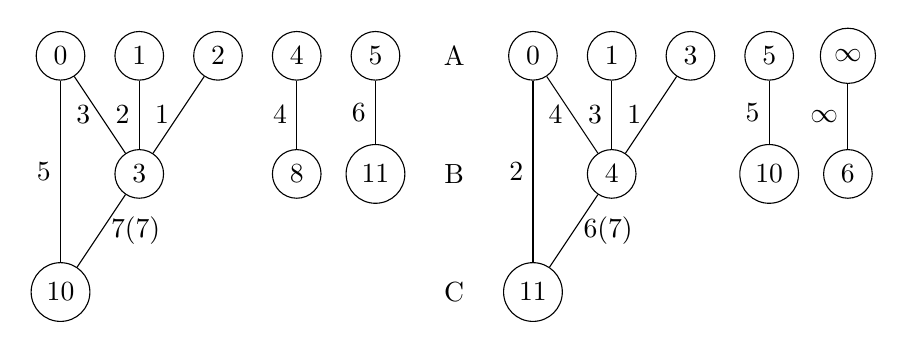
\begin{tikzpicture}[baseline={(current bounding box.center)}]
        \node [draw, circle] (0) at (0,0) {0};
        \node [draw, circle] (1) at (1,0) {1};
        \node [draw, circle] (2) at (2,0) {2};
        \node [draw, circle] (4) at (3,0) {4};
        \node [draw, circle] (5) at (4,0) {5};
        \node [draw, circle] (3) at (1,-1.5) {3};
        \node [draw, circle] (8) at (3,-1.5) {8};
        \node [draw, circle] (11) at (4,-1.5) {11};
        \node [draw, circle] (10) at (0,-3) {10};
        \node (A) at (5,0) {A};
        \node (B) at (5,-1.5) {B};
        \node (C) at (5,-3) {C};

        \draw (0) -- node [midway, left] {5} (10);
        \draw (0) -- node [midway,left] {3} (3);
        \draw (3) --node [midway,left] {2} (1);
        \draw (3) -- node [midway, left] {1} (2);
        \draw (4) -- node [midway, left] {4} (8);
        \draw (5) -- node [midway, left] {6} (11);
        \draw (3) -- node [midway, right] {7(7)} (10);
    
        \node [draw, circle] (0) at (6,0) {0};
        \node [draw, circle] (1) at (7,0) {1};
        \node [draw, circle] (2) at (8,0) {3};
        \node [draw, circle] (4) at (9,0) {5};
        \node [draw, circle] (5) at (10,0) {$\infty$};
        \node [draw, circle] (3) at (7,-1.5) {4};
        \node [draw, circle] (8) at (9,-1.5) {10};
        \node [draw, circle] (11) at (10,-1.5) {6};
        \node [draw, circle] (10) at (6,-3) {11};
        \draw (0) -- node [midway, left] {2} (10);
        \draw (0) -- node [midway,left] {4} (3);
        \draw (3) --node [midway,left] {3} (1);
        \draw (3) -- node [midway, left] {1} (2);
        \draw (4) -- node [midway, left] {5} (8);
        \draw (5) -- node [midway, left] {$\infty$} (11);
        \draw (3) -- node [midway, right] {6(7)} (10);
    \end{tikzpicture}
    \vskip20pt
    
    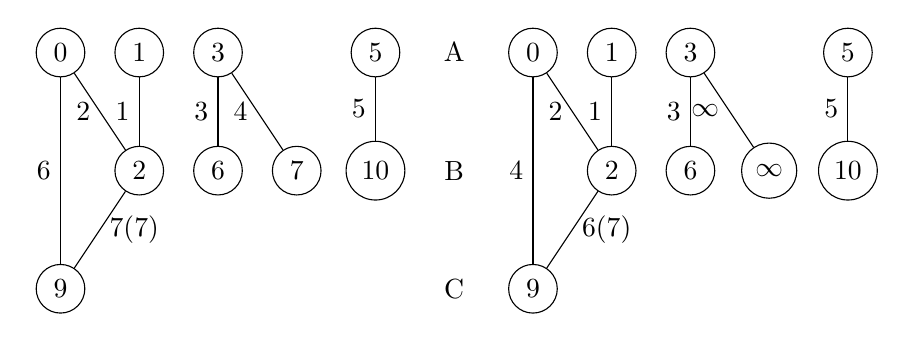
\begin{tikzpicture}[baseline={(current bounding box.center)}]
        \node [draw, circle] (0) at (0,0) {0};
        \node [draw, circle] (2) at (1,-1.5) {2};
        \node [draw, circle] (9) at (0,-3) {9};
        \node [draw, circle] (1) at (1,0) {1};
        \node [draw, circle] (3) at (2,0) {3};
        \node [draw, circle] (6) at (2,-1.5) {6};
        \node [draw, circle] (7) at (3,-1.5) {7};
        \node [draw, circle] (5) at (4,0) {5};
        \node [draw, circle] (10) at (4,-1.5) {10};
        \node (A) at (5,0) {A};
        \node (B) at (5,-1.5) {B};
        \node (C) at (5,-3) {C};
        \draw (0) -- node [midway, left] {6} (9);
        \draw (0) -- node [midway, left] {2} (2);
        \draw (2) -- node [midway, left] {1} (1);
        \draw (2) -- node [midway, right] {7(7)} (9);
        \draw (3) -- node [midway, left] {3} (6);
        \draw (3) -- node [midway, left] {4} (7);
        \draw (5) --node [midway, left] {5} (10);
    
        \node [draw, circle] (0) at (6,0) {0};
        \node [draw, circle] (2) at (7,-1.5) {2};
        \node [draw, circle] (9) at (6,-3) {9};
        \node [draw, circle] (1) at (7,0) {1};
        \node [draw, circle] (3) at (8,0) {3};
        \node [draw, circle] (6) at (8,-1.5) {6};
        \node [draw, circle] (7) at (9,-1.5) {$\infty$};
        \node [draw, circle] (5) at (10,0) {5};
        \node [draw, circle] (10) at (10,-1.5) {10};
        \draw (0) -- node [midway, left] {4} (9);
        \draw (0) -- node [midway, left] {2} (2);
        \draw (2) -- node [midway, left] {1} (1);
        \draw (2) -- node [midway, right] {6(7)} (9);
        \draw (3) -- node [midway, left] {3} (6);
        \draw (3) -- node [midway, left] {$\infty$} (7);
        \draw (5) --node [midway, left] {5} (10);
    \end{tikzpicture}
    \vskip20pt
    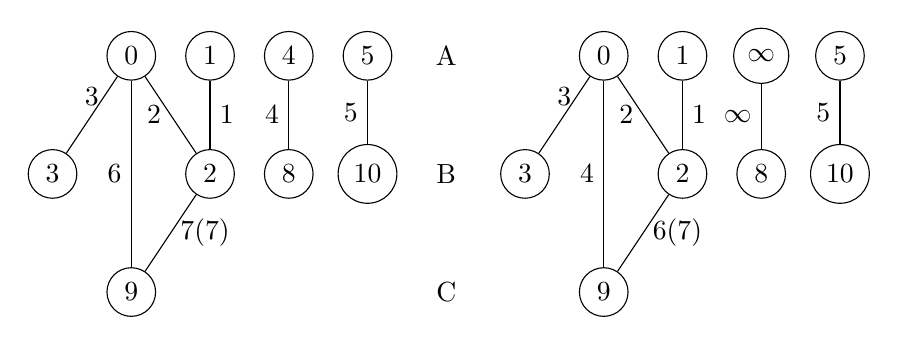
\begin{tikzpicture}[baseline={(current bounding box.center)}]
        \node (A) at (5,0) {A};
        \node (B) at (5,-1.5) {B};
        \node (C) at (5,-3) {C};
        
        \node [draw, circle] (0) at (1,0) {0};
        \node [draw, circle] (2) at (2,-1.5) {2};
        \node [draw, circle] (9) at (1,-3) {9};
        \node [draw, circle] (1) at (2,0) {1};
        \node [draw, circle] (3) at (0,-1.5) {3};
        \node [draw, circle] (4) at (3,0) {4};
        \node [draw, circle] (5) at (4,0) {5};
        \node [draw, circle] (8) at (3,-1.5) {8};
        \node [draw, circle] (10) at (4,-1.5) {10};
 
        \draw (0) -- node [midway, above] {3} (3);
        \draw (2) -- node[midway, right] {1} (1);
        \draw (0) -- node [midway, left] {6} (9);
        \draw (2) -- node [midway, right] {7(7)} (9);
        \draw (4) -- node [midway, left] {4} (8);
        \draw (5) -- node [midway, left] {5} (10);
        \draw (0) -- node [midway, left] {2} (2);
    
        \node [draw, circle] (0) at (7,0) {0};
        \node [draw, circle] (2) at (8,-1.5) {2};
        \node [draw, circle] (9) at (7,-3) {9};
        \node [draw, circle] (1) at (8,0) {1};
        \node [draw, circle] (3) at (6,-1.5) {3};
        \node [draw, circle] (4) at (9,0) {$\infty$};
        \node [draw, circle] (5) at (10,0) {5};
        \node [draw, circle] (8) at (9,-1.5) {8};
        \node [draw, circle] (10) at (10,-1.5) {10};

        \draw (0) -- node [midway, above] {3} (3);
        \draw (2) -- node[midway, right] {1} (1);
        \draw (0) -- node [midway, left] {4} (9);
        \draw (2) -- node [midway, right] {6(7)} (9);
        \draw (4) -- node [midway, left] {$\infty$} (8);
        \draw (5) -- node [midway, left] {5} (10);
        \draw (0) -- node [midway, left] {2} (2);
    \end{tikzpicture}
    \vskip20pt
    \caption{Labeled Graphs}
    \label{fig:label}
\end{figure}

\newpage

\begin{figure}[H]
    \centering
    % First picture
    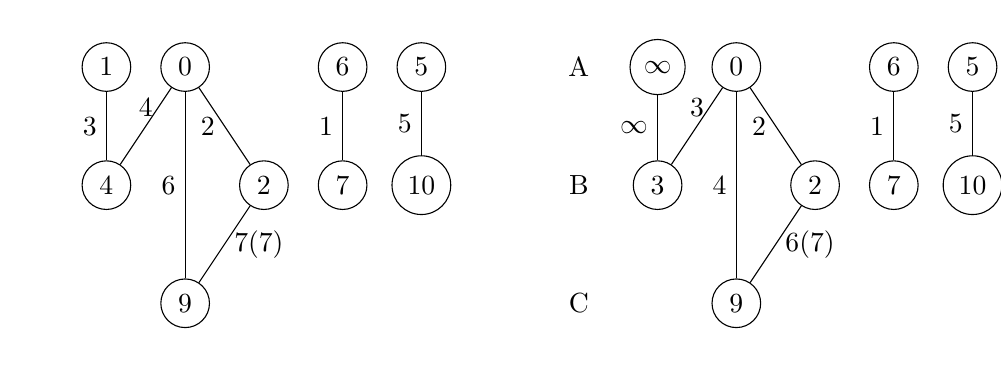
\begin{tikzpicture}[baseline=(A.base)]
        \useasboundingbox (-2,-3.5) rectangle (10,0.5);
        \node (A) at (5,0) {A};
        \node (B) at (5,-1.5) {B};
        \node (C) at (5,-3) {C};
    
        \node [draw, circle] (0) at (0,0) {0};
        \node [draw, circle] (2) at (1,-1.5) {2};
        \node [draw, circle] (9) at (0,-3) {9};
        \node [draw, circle] (1) at (-1,0) {1};
        \node [draw, circle] (4) at (-1,-1.5) {4};
        \node [draw, circle] (6) at (2,0) {6};
        \node [draw, circle] (7) at (2,-1.5) {7};
        \node [draw, circle] (5) at (3,0) {5};
        \node [draw, circle] (10) at (3,-1.5) {10};
    
        \draw (0) -- node [midway, left] {2} (2);
        \draw (0) -- node [midway, left] {6} (9);
        \draw (9) -- node [midway, right] {7(7)} (2);
        \draw (0) -- node [midway,above] {4} (4);
        \draw (4) -- node [midway, left] {3} (1);
        \draw (6) -- node [midway,left] {1} (7);
        \draw (5) -- node [midway,left] {5} (10);
    
        \node [draw, circle] (0b) at (7,0) {0};
        \node [draw, circle] (2b) at (8,-1.5) {2};
        \node [draw, circle] (9b) at (7,-3) {9};
        \node [draw, circle] (1b) at (6,0) {$\infty$};
        \node [draw, circle] (4b) at (6,-1.5) {3};
    
        \node [draw, circle] (6b) at (9,0) {6};
        \node [draw, circle] (7b) at (9,-1.5) {7};
    
        \node [draw, circle] (5b) at (10,0) {5};
        \node [draw, circle] (10b) at (10,-1.5) {10};
    
        \draw (0b) -- node [midway, left] {2} (2b);
        \draw (0b) -- node [midway, left] {4} (9b);
        \draw (9b) -- node [midway, right] {6(7)} (2b);
        \draw (0b) -- node [midway,above] {3} (4b);
        \draw (4b) -- node [midway, left] {$\infty$} (1b);
        \draw (6b) -- node [midway,left] {1} (7b);
        \draw (5b) -- node [midway,left] {5} (10b);
    \end{tikzpicture}
    
    \vskip20pt
    
    % Second picture
    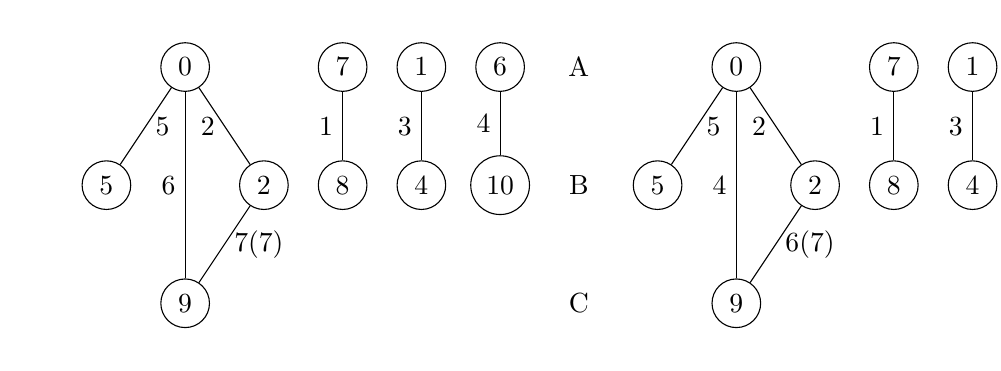
\begin{tikzpicture}[baseline=(A.base)]
        \useasboundingbox (-2,-3.5) rectangle (10,0.5);
        \node (A) at (5,0) {A};
        \node (B) at (5,-1.5) {B};
        \node (C) at (5,-3) {C};
    
        \node [draw, circle] (0) at (0,0) {0};
        \node [draw, circle] (2) at (1,-1.5) {2};
        \node [draw, circle] (9) at (0,-3) {9};
        \node [draw, circle] (5) at (-1,-1.5) {5};
    
        \node [draw, circle] (7) at (2,0) {7};
        \node [draw, circle] (8) at (2,-1.5) {8};
    
        \node [draw, circle] (1) at (3,0) {1};
        \node [draw, circle] (4) at (3,-1.5) {4};
    
        \node [draw, circle] (6) at (4,0) {6};
        \node [draw, circle] (10) at (4,-1.5) {10};
    
        \draw (0) -- node [midway, left] {6} (9);
        \draw (0) -- node [midway, left] {2} (2);
        \draw (7) -- node [midway, left] {1} (8);
        \draw (1) -- node [midway, left] {3} (4);
        \draw (6) -- node [midway, left] {4} (10);
        \draw (2) -- node [midway, right] {7(7)} (9);
        \draw (0) -- node [midway, right] {5} (5);
    
        \node [draw, circle] (5b) at (6,-1.5) {5};
        \node [draw, circle] (0b) at (7,0) {0};
        \node [draw, circle] (2b) at (8,-1.5) {2};
        \node [draw, circle] (9b) at (7,-3) {9};
    
        \node [draw, circle] (7b) at (9,0) {7};
        \node [draw, circle] (8b) at (9,-1.5) {8};
    
        \node [draw, circle] (1b) at (10,0) {1};
        \node [draw, circle] (4b) at (10,-1.5) {4};
    
        \node [draw, circle] (6b) at (11,0) {$\infty$};
        \node [draw, circle] (10b) at (11,-1.5) {10};
    
        \draw (0b) -- node [midway, left] {4} (9b);
        \draw (0b) -- node [midway, left] {2} (2b);
        \draw (7b) -- node [midway, left] {1} (8b);
        \draw (1b) -- node [midway, left] {3} (4b);
        \draw (6b) -- node [midway, left] {$\infty$} (10b);
        \draw (2b) -- node [midway, right] {6(7)} (9b);
        \draw (0b) -- node [midway, right] {5} (5b);
    \end{tikzpicture}
    
    \caption{Labeled Graphs}
    \label{fig:label}
    \end{figure}
    

\newpage

\begin{figure}[H]
    \centering
    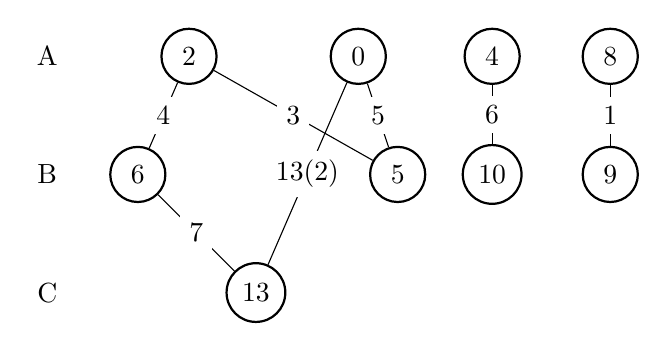
\begin{tikzpicture}[roundnode/.style={circle, draw=black, fill=black!0, thick, minimum size=7mm}] 
        \node[] (A1) at (-.15,4) {A};
        \node[] (B1) at (-.15,2.5) {B};
        \node[] (C1) at (-.15,1) {C};
        \node[roundnode] (A) at (1.65,4) {2};
        \node[roundnode] (B) at (1,2.5) {6};
        \node[roundnode] (C) at (2.5,1) {13};
        \node[roundnode] (D) at (3.8,4) {0};
        \node[roundnode] (E) at (4.3,2.5) {5};
        \node[roundnode] (F) at (5.5,4) {4};
        \node[roundnode] (G) at (5.5,2.5) {10};
        \node[roundnode] (H) at (7,2.5) {9};
        \node[roundnode] (I) at (7,4) {8};
        
        \tikzset{mystyle/.style={->,double=orange}} 
        \tikzset{every node/.style={fill=white}}
        
        \draw[-] (A) edge[] node {$4$} (B);
        \draw[-] (B) edge[] node {$7$} (C);
        \draw[-] (C) edge[] node {$13(2)$} (D);
        \draw[-] (D) edge[] node {$5$} (E);
        \draw[-] (E) edge[] node {$3$} (A);
        \draw[-] (F) edge[] node {$6$} (G);
        \draw[-] (H) edge[] node {$1$} (I);

    \end{tikzpicture}
    \caption{$\rho$-tripartite labeling}
    \label{fig:rhoLabelingsTripartite}
\end{figure}

\begin{figure}[H]
    \centering
        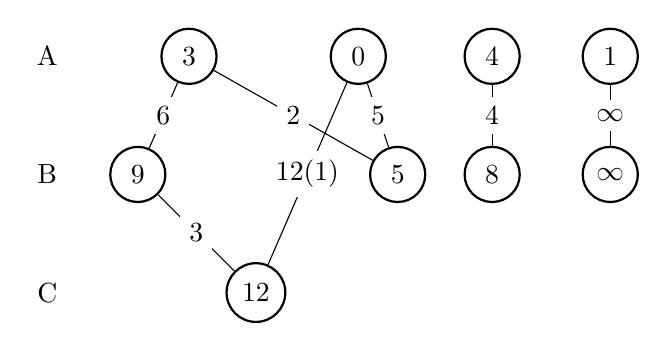
\begin{tikzpicture}[roundnode/.style={circle, draw=black, fill=black!0, thick, minimum size=7mm}] 
            \node[] (A1) at (-.15,4) {A};
            \node[] (B1) at (-.15,2.5) {B};
            \node[] (C1) at (-.15,1) {C};
            \node[roundnode] (A) at (1.65,4) {3};
            \node[roundnode] (B) at (1,2.5) {9};
            \node[roundnode] (C) at (2.5,1) {12};
            \node[roundnode] (D) at (3.8,4) {0};
            \node[roundnode] (E) at (4.3,2.5) {5};
            \node[roundnode] (F) at (5.5,4) {4};
            \node[roundnode] (G) at (5.5,2.5) {8};
            \node[roundnode] (H) at (7,2.5) {$\infty$};
            \node[roundnode] (I) at (7,4) {1};
            
            \tikzset{mystyle/.style={->,double=orange}} 
            \tikzset{every node/.style={fill=white}}
            
            \draw[-] (A) edge[] node {$6$} (B);
            \draw[-] (B) edge[] node {$3$} (C);
            \draw[-] (C) edge[] node {$12(1)$} (D);
            \draw[-] (D) edge[] node {$5$} (E);
            \draw[-] (E) edge[] node {$2$} (A);
            \draw[-] (F) edge[] node {$4$} (G);
            \draw[-] (H) edge[] node {$\infty$} (I);

        \end{tikzpicture}
    \caption{1-rotational $\rho$-tripartite labeling}
    \label{fig:oneRotationalRhoTrip}
\end{figure}
\newpage

In Figure \ref{fig:rhoLabelingBipartite} we show the ordered $\rho$-labelings of graphs $G_1$,$G_2$, and $G_3$.

\begin{figure}[H]
    \centering

        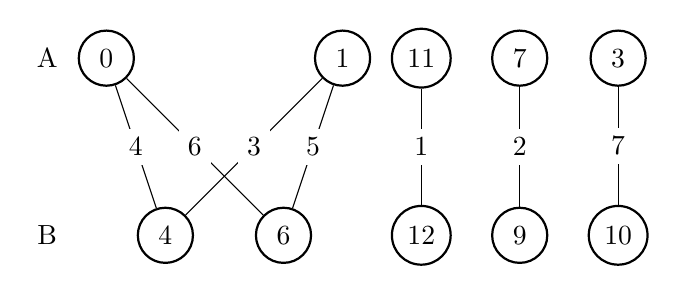
\begin{tikzpicture}[roundnode/.style={circle, draw=black, fill=black!0, thick, minimum size=7mm}] 
            \node[] (A1) at (-1,2.25) {A};
            \node[] (C1) at (-1,0) {B};
            \node[roundnode] (A) at (0.5,0) {4};
            \node[roundnode] (B) at (-.25,2.25) {0};
            \node[roundnode] (C) at (2,0) {6};
            \node[roundnode] (D) at (2.75,2.25) {1};
            \node[roundnode] (E) at (3.75,2.25) {11};
            \node[roundnode] (F) at (3.75,0) {12};
            \node[roundnode] (G) at (5,2.25) {7};
            \node[roundnode] (H) at (5,0) {9};
            \node[roundnode] (I) at (6.25,2.25) {3};
            \node[roundnode] (J) at (6.25,0) {10};
            
            
            \tikzset{mystyle/.style={->,double=orange}} 
            \tikzset{every node/.style={fill=white}}
            
            \draw[-] (A) edge[] node {$4$} (B);
            \draw[-] (B) edge[] node {$6$} (C);
            \draw[-] (C) edge[] node {$5$} (D);
            \draw[-] (D) edge[] node {$3$} (A);
            \draw[-] (E) edge[] node {$1$} (F);
            \draw[-] (G) edge[] node {$2$} (H);
            \draw[-] (I) edge[] node {$7$} (J);

        \end{tikzpicture}

        \vskip20pt

        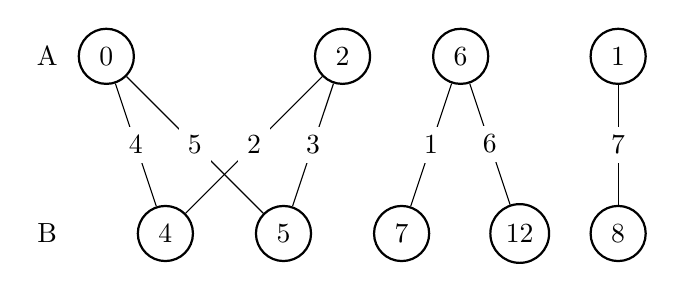
\begin{tikzpicture}[
        roundnode/.style={circle, draw=black, fill=black!0, thick, minimum size=7mm}
        ] 
            \node[] (A1) at (-1,2.25) {A};
            \node[] (C1) at (-1,0) {B};
            \node[roundnode] (A) at (0.5,0) {4};
            \node[roundnode] (B) at (-.25,2.25) {0};
            \node[roundnode] (C) at (2,0) {5};
            \node[roundnode] (D) at (2.75,2.25) {2};
            \node[roundnode] (E) at (4.25,2.25) {6};
            \node[roundnode] (F) at (3.5,0) {7};
            \node[roundnode] (G) at (5,0) {12};
            \node[roundnode] (H) at (6.25,2.25) {1};
            \node[roundnode] (I) at (6.25,0) {8};
            
            \tikzset{mystyle/.style={->,double=orange}} 
            \tikzset{every node/.style={fill=white}}
            
            \draw[-] (A) edge[] node {$4$} (B);
            \draw[-] (B) edge[] node {$5$} (C);
            \draw[-] (C) edge[] node {$3$} (D);
            \draw[-] (D) edge[] node {$2$} (A);
            \draw[-] (E) edge[] node {$1$} (F);
            \draw[-] (E) edge[] node {$6$} (G);
            \draw[-] (H) edge[] node {$7$} (I);

        \end{tikzpicture}

        \vskip20pt

        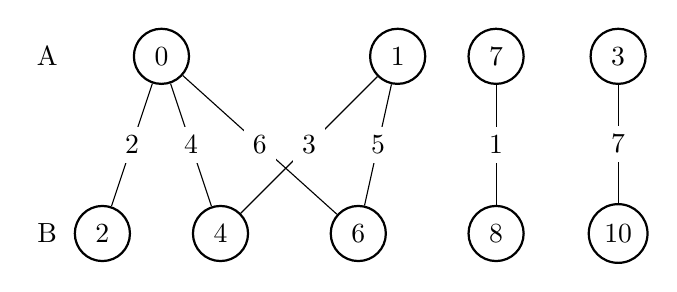
\begin{tikzpicture}[
        roundnode/.style={circle, draw=black, fill=black!0, thick, minimum size=7mm}
        ] 
            \node[] (A1) at (-2.2,2.25) {A};
            \node[] (C1) at (-2.2,0) {B};
            \node[roundnode] (A) at (0,0) {4};
            \node[roundnode] (B) at (-.75,2.25) {0};
            \node[roundnode] (C) at (-1.5,0) {2};
            \node[roundnode] (D) at (1.75,0) {6};
            \node[roundnode] (E) at (2.25,2.25) {1};
            \node[roundnode] (F) at (3.5,0) {8};
            \node[roundnode] (G) at (3.5,2.25) {7};
            \node[roundnode] (H) at (5.05,0) {10};
            \node[roundnode] (I) at (5.05,2.25) {3};
            
            \tikzset{mystyle/.style={->,double=orange}} 
            \tikzset{every node/.style={fill=white}}
            
            \draw[-] (A) edge[] node {$4$} (B);
            \draw[-] (B) edge[] node {$2$} (C);
            \draw[-] (B) edge[] node {$6$} (D);
            \draw[-] (D) edge[] node {$5$} (E);
            \draw[-] (E) edge[] node {$3$} (A);
            \draw[-] (F) edge[] node {$1$} (G);
            \draw[-] (H) edge[] node {$7$} (I);

        \end{tikzpicture}

    
    \caption{Ordered $\rho$-labelings}
    \label{fig:rhoLabelingBipartite}
\end{figure}
\newpage

In Figure \ref{fig:oneRotationalRhoBip} we show 1-rotational ordered $\rho$-labelings of $G_1$, $G_2$, and $G_3$.
\begin{figure}[H]
    \centering

        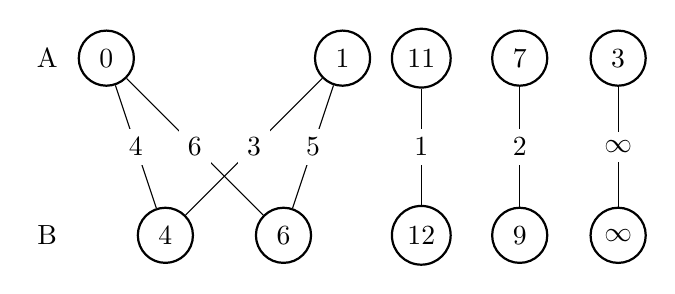
\begin{tikzpicture}[roundnode/.style={circle, draw=black, fill=black!0, thick, minimum size=7mm}] 
            \node[] (A1) at (-1,2.25) {A};
            \node[] (C1) at (-1,0) {B};
            \node[roundnode] (A) at (0.5,0) {4};
            \node[roundnode] (B) at (-.25,2.25) {0};
            \node[roundnode] (C) at (2,0) {6};
            \node[roundnode] (D) at (2.75,2.25) {1};
            \node[roundnode] (E) at (3.75,2.25) {11};
            \node[roundnode] (F) at (3.75,0) {12};
            \node[roundnode] (G) at (5,2.25) {7};
            \node[roundnode] (H) at (5,0) {9};
            \node[roundnode] (I) at (6.25,2.25) {3};
            \node[roundnode] (J) at (6.25,0) {$\infty$};
            
            
            \tikzset{mystyle/.style={->,double=orange}} 
            \tikzset{every node/.style={fill=white}}
            
            \draw[-] (A) edge[] node {$4$} (B);
            \draw[-] (B) edge[] node {$6$} (C);
            \draw[-] (C) edge[] node {$5$} (D);
            \draw[-] (D) edge[] node {$3$} (A);
            \draw[-] (E) edge[] node {$1$} (F);
            \draw[-] (G) edge[] node {$2$} (H);
            \draw[-] (I) edge[] node {$\infty$} (J);

        \end{tikzpicture}

        \vskip20pt

        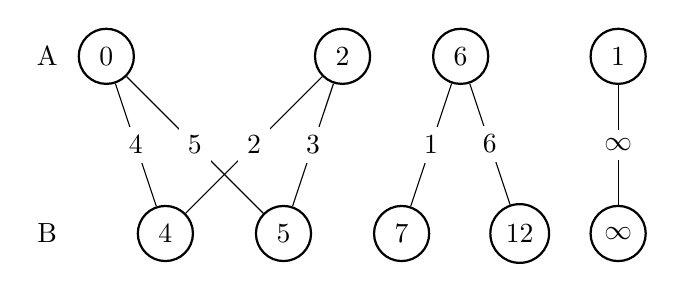
\begin{tikzpicture}[roundnode/.style={circle, draw=black, fill=black!0, thick, minimum size=7mm}] 
            \node[] (A1) at (-1,2.25) {A};
            \node[] (C1) at (-1,0) {B};
            \node[roundnode] (A) at (0.5,0) {4};
            \node[roundnode] (B) at (-.25,2.25) {0};
            \node[roundnode] (C) at (2,0) {5};
            \node[roundnode] (D) at (2.75,2.25) {2};
            \node[roundnode] (E) at (4.25,2.25) {6};
            \node[roundnode] (F) at (3.5,0) {7};
            \node[roundnode] (G) at (5,0) {12};
            \node[roundnode] (H) at (6.25,2.25) {1};
            \node[roundnode] (I) at (6.25,0) {$\infty$};
            
            \tikzset{mystyle/.style={->,double=orange}} 
            \tikzset{every node/.style={fill=white}}
            
            \draw[-] (A) edge[] node {$4$} (B);
            \draw[-] (B) edge[] node {$5$} (C);
            \draw[-] (C) edge[] node {$3$} (D);
            \draw[-] (D) edge[] node {$2$} (A);
            \draw[-] (E) edge[] node {$1$} (F);
            \draw[-] (E) edge[] node {$6$} (G);
            \draw[-] (H) edge[] node {$\infty$} (I);

        \end{tikzpicture}
        \vskip20pt
        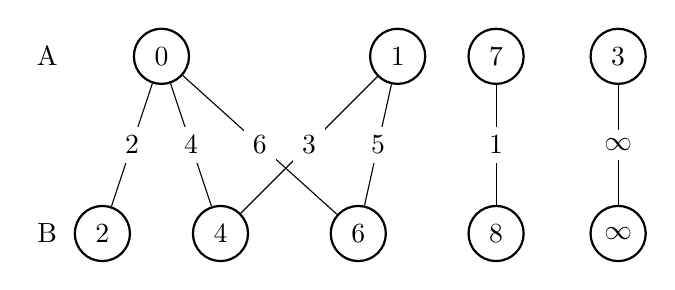
\begin{tikzpicture}[roundnode/.style={circle, draw=black, fill=black!0, thick, minimum size=7mm}] 
            \node[] (A1) at (-2.2,2.25) {A};
            \node[] (C1) at (-2.2,0) {B};
            \node[roundnode] (A) at (0,0) {4};
            \node[roundnode] (B) at (-.75,2.25) {0};
            \node[roundnode] (C) at (-1.5,0) {2};
            \node[roundnode] (D) at (1.75,0) {6};
            \node[roundnode] (E) at (2.25,2.25) {1};
            \node[roundnode] (F) at (3.5,0) {8};
            \node[roundnode] (G) at (3.5,2.25) {7};
            \node[roundnode] (H) at (5.05,0) {$\infty$};
            \node[roundnode] (I) at (5.05,2.25) {3};
            
            \tikzset{mystyle/.style={->,double=orange}} 
            \tikzset{every node/.style={fill=white}}
            
            \draw[-] (A) edge[] node {$4$} (B);
            \draw[-] (B) edge[] node {$2$} (C);
            \draw[-] (B) edge[] node {$6$} (D);
            \draw[-] (D) edge[] node {$5$} (E);
            \draw[-] (E) edge[] node {$3$} (A);
            \draw[-] (F) edge[] node {$1$} (G);
            \draw[-] (H) edge[] node {$\infty$} (I);

        \end{tikzpicture}

    \caption{1-rotational ordered $\rho$-labeling}
    \label{fig:oneRotationalRhoBip}
\end{figure}
\end{document}
